%-*- program: biber -*-`    
\documentclass{mekit17}
\usepackage[utf8]{inputenc}
\usepackage[english]{babel}
\usepackage{lmodern} % use this to fix errors with \scriptsize (used in header on page 1)

% \usepackage[parfill]{parskip}
\usepackage[euler]{textgreek} % option "euler" uses Euler fonts as a companion for all fonts except Helvetica -- this is the default LaTeX-font for greek symbols as far as I can see

% biber/biblatex  - - - - - - - - - - - - - - - - - - - - - - - - - - - - - - - - - - - - - - - - %
\usepackage{csquotes} % required by {babel} (or biblatex?)
\usepackage[%
    backend=biber,  % biblatex is the package, biber is the (default). The alternative is backend=bibtex, but biber should be better.
    % sorting=nyt,    %
    sorting=none, % in order of citation
%    style=numeric,  %
    style=numeric-comp,
    %firstinits=true % render all first and middle names as initials
    giveninits=true,
    maxbibnames=99 % show all names in bibliography
]{biblatex} % Note that "sorting=none" is NOT the same as leaving the field blank, "sorting=none" means "sorting=citeorder".
% About DATES:
% The date fields date, origdate, eventdate, and urldate require a date specification in yyyy-mm-dd format. Date ranges are given as yyyy-mm-dd/yyyy-mm-dd. Partial dates are valid provided that date components are omitted at the end only. You may specify an open ended date range by giving the range separator and omitting the end date (e. g., yyyy/).

% Example from here: http://codydunne.blogspot.no/2012/01/suppressing-bibtex-fields-for-specific.html
\AtEveryBibitem{% Clean up the bibtex rather than editing it
    \clearlist{address}
%  \clearfield{date}
%     \ifentrytype{www}{}{ % url is alias for ``online''
%         \clearfield{url}
%     }
    \ifentrytype{online}{}{
        \clearfield{url}
    }
    \clearfield{doi}
    \clearfield{eprint}
    \clearfield{isbn}
    \clearfield{issn}
    \clearlist{location}
    \clearfield{month}
    \clearfield{series}
    
    \ifentrytype{book}{}{% Remove publisher and editor except for books
        % \clearlist{publisher}
        % \clearname{editor}
        \clearfield{pages}
    }
}

\usepackage{amsmath}
\usepackage{amsfonts}
\usepackage{amssymb}
\usepackage{bm} % bold math
\usepackage{commath2,commath2-additions}
% \usepackage{cancel} % strikethrough/cancel equations
% \usepackage{authblk} % author/affiliation..?
\usepackage{import}
\usepackage{graphicx}
% \usepackage[font=small,labelfont=bf,width=.9\textwidth]{caption}
\usepackage[textwidth=2.5cm,disable]{todonotes}
\newcommand{\inlinetodo}[1]{\todo[inline]{#1}}
\usepackage[section]{placeins} % forces floats (images) to stay within their section (stops results images from flowing into conclusion)
\usepackage{siunitx}
\sisetup{%
    load-configurations = abbreviations, %
    per-mode = symbol, %
    % range-phrase = -- %
}%
\usepackage{booktabs} % better tables, \hline --> \toprule, \midrule, \bottomrule
\usepackage{multirow}
\usepackage{printlen} % to print lengths like \textwidth, \textheight using \printlength{\textwidth}
\uselengthunit{mm}
% \usepackage{subcaption}
\usepackage{pbox}

% highlighting
\usepackage{color} % Must be loaded before soul, for highligting
\usepackage{soul}
\usepackage{xcolor}
\newcommand{\redtext}[1]{\textcolor{red}{#1}}
% \renewcommand{\hl}[2][yellow]{%
%     \sethlcolor{#1}%
%     \hl{#2}%
% }%
\DeclareRobustCommand{\hlg}[1]{%
    \sethlcolor{green}%
    \hl{#1}%
}%
\DeclareRobustCommand{\hly}[1]{%
    \sethlcolor{yellow}%
    \hl{#1}%
}%
% \newcommand{\greenbox}[1]{\colorbox{green}{#1}}
% \newcommand{\yellowbox}[1]{\colorbox{yellow}{#1}}
\newcommand{\greenbox}[1]{\hlg{#1}}
\newcommand{\yellowbox}[1]{\hly{#1}}

\usepackage{hyperref}
\usepackage{cleveref}

% Custom bracket sizes \vast and \Vast
\makeatletter
\newcommand{\vast}{\bBigg@{3}}
\newcommand{\Vast}{\bBigg@{4}}
\makeatother

% math symbols
\renewcommand{\textmu}{\textmugreek}
\newcommand{\bvec}[1]{\bm{#1}}
\renewcommand{\vec}[1]{\bvec{#1}}
\newcommand{\vect}[1]{\bm{#1}}
\newcommand{\upmu}{\textup{\textmu}}
\newcommand*{\epsO}{\epsilon_0}
\let\div\olddiv
\DeclareMathOperator{\div}{div}
\let\oldtimes\times
\let\times\cdot
% \DeclareMathOperator{\abs}{abs}
\newcommand{\overbar}[1]{\mkern 1.5mu\overline{\mkern-1.5mu#1\mkern-1.5mu}\mkern 1.5mu}

% \newcommand{\Reyn}{\operatorname{\mathit{R\kern-.04em e}}} % Reynolds number
% \newcommand{\Nuss}{\operatorname{\mathit{N\kern-.09em u}}} % Nusselt number
% \newcommand{\Pran}{\operatorname{\mathit{P\kern-.03em r}}} % Prandtl number

\newcommand{\Reyn}{\operatorname{R\kern-.04em e}} % Reynolds number
\newcommand{\Nuss}{\operatorname{N\kern-.09em u}} % Nusselt number
\newcommand{\Pran}{\operatorname{P\kern-.03em r}} % Prandtl number
% % http://tex.stackexchange.com/a/175105/31078

% colored tables
\usepackage{tikz}
\usepackage{collcell}

% the min, mid and max values
\newcommand*{\MinNumberA}{0.0030}%
\newcommand*{\MaxNumberA}{1.3207 }%
% \newcommand*{\MinNumberB}{0.0}%
% \newcommand*{\MaxNumberB}{2.7952}%
\newcommand*{\MinNumberC}{0.0}%
\newcommand*{\MaxNumberC}{0.1579}%

% apply the gradient macro
\newcommand{\ApplyGradientA}[1]{%
    \pgfmathsetmacro{\PercentColor}{%
        max(%
            min(%
                100.0*(\MaxNumber - #1)/(\MaxNumberA - \MinNumberA),%
                100.0%
            ),%
            0.00%
        )%
    } %
    \hspace{-0.33em}\colorbox{white!\PercentColor!green}{#1}
}

% \newcommand{\ApplyGradientB}[1]{%
%     \pgfmathsetmacro{\PercentColor}{%
%         max(%
%             min(%
%                 100.0*(\MaxNumber - #1)/(\MaxNumberB - \MinNumberB),%
%                 100.0%
%             ),%
%             0.00%
%         )%
%     } %
%     \hspace{-0.33em}\colorbox{white!\PercentColor!green}{#1}
% }

\newcommand{\ApplyGradientC}[1]{%
    \pgfmathsetmacro{\PercentColor}{%
        max(%
            min(%
                100.0*(\MaxNumber - #1)/(\MaxNumberC - \MinNumberC),%
                100.0%
            ),%
            0.00%
        )%
    } %
    \hspace{-0.33em}\colorbox{white!\PercentColor!green}{#1}
}

\newcolumntype{R}{>{\collectcell\ApplyGradientA}c<{\endcollectcell}}
% \newcolumntype{R2}{>{\collectcell\ApplyGradientB}c<{\endcollectcell}}
\newcolumntype{T}{>{\collectcell\ApplyGradientC}c<{\endcollectcell}}

% \renewcommand{\arraystretch}{0}
% \setlength{\fboxsep}{3mm} % box size
% \setlength{\tabcolsep}{0pt}

\addbibresource{remote.bib}

% \title{The relative importance of model parameters in predictive transient models}
\title{THE RELATIVE IMPORTANCE OF MODEL PARAMETERS IN PREDICTIVE TRANSIENT MODELS}

\author{Filip Sund$^{1,2}$}

\heading{Filip Sund}

\address{%
$^{1}$Norwegian University of Science and Technology \\
Department of Energy and Process Engineering\\
7491 Trondheim, Norway
\and%
$^{2}$Uni Research Polytec\\
5527 Haugesund, Norway \\
e-mail: filip.sund@polytec.no}

\keywords{Computational Methods}

\abstract{\textit{A sensitivity study on numerical transient flow models for compressible gas was performed to determine the most important parameters when simulating long offshore gas pipelines. A simplified pipeline was simulated with synthetic transient boundary conditions, while systematically modifying different model parameters and correlations. It was found that, for the mass flow and pressure, the most important parameters, \redtext{by a large margin}, are the friction factor and the compressibility factor. \redtext{Further, after a long offshore section, none of the parameters has much impact on the temperature. In addition it was found that on shore, buried under ground, and initially after going offshore, the most important parameters for the temperature are the gas heat capacity, the compressibility factor and its derivatives, and the friction factor.}}}

\begin{document}
% \maketitle

% \uselengthunit{mm}
% \printlength{\textheight}
% \printlength{\textwidth}

% \uselengthunit{in}
% \printlength{\textheight}
% \printlength{\textwidth}

% \section{Introduction}
\section{INTRODUCTION}
Natural gas exported from Norway to Europe accounts for around 25 percent of the yearly gas consumption in the European Union\todo{source?}. The gas is transported from Norway through pipelines that are up to 1166 km long. %
To ensure that the pipelines stay within their operating limits, to monitor the pipelines for leaks, and to track changes in gas quality, %
it is important to know the state of the gas in the pipelines. %
But measurements of the state of the gas are only available at the inlet and outlet, which means that \redtext{numerical} models are necessary to know the state of the gas between the endpoints. 

Simulating compressible gas flow is a highly complex issue, so to reduce the problem to a tractable one, several empirical relations and correlations like the Colebrook-White equation and the Dittus-Boelter equation are typically used to describe different aspects of the system. When doing this errors are introduced into the simulations, the total effect of which can be hard to calculate a priori, and which will depend on the state and system being simulated. 

The objective of this study is to investigate which parameters and correlations in the gas models that have greatest impact on the modelled results, especially during transient conditions, to know where to apply effort when trying to improve the models. A similar study limited to steady state models was done by Langelandsvik \cite{Langelandsvik2008Modeling}, and some work using transient models was by Helgaker \cite{Helgaker2013Modeling}. The present work deals with transient one-dimensional non-isothermal models for compressible natural gas mixtures, and a simplified pipeline is modelled using synthetic but representative flow transients as boundary conditions.

This article is structured as follows: The theoretical foundation and underlying equations are presented in \Cref{theory}
%The numerical scheme is presented in \cref{num} 
followed by the presentation of the studied pipeline system in \cref{simulations}. Results are presented and discussed in \cref{results} while concluding remarks are drawn in \cref{conclusion}.

% \section{Theory}
\section{THEORY}
\label{theory}
The description of the theoretical foundation closely follows the description in \cite{Chaczykowski2017}. 

\subsection{Conservation laws}
The governing equations for compressible, non-isothermal, transient pipeline gas flow \hlbr{are derived by averaging the Reynolds time-averaged conservation laws for viscous flow over the cross-section, resulting in:} \\\\
the \textbf{continuity equation}
\begin{align}
    \pdt{\rho} + \pdx{(\rho u)} = 0
, \label{eq:contEq}
\end{align}
the \textbf{momentum equation} \cite{Daneshyar1976OneDimensional}
\begin{align}
    \rho\del{\pdt{u} + u \pdx{u}} + \pdx{p} = -\frac{f\rho \abs{u} u}{2D} - \rho g \sin \theta
, \label{eq:momEq}
\end{align}
and the \textbf{energy equation} \cite{White2006Viscous}
\begin{align}
    \rho\del{\pdt{e} + u\pdx{e}} + p\pdx{u} = \frac{f\rho u^3}{2D} + \frac{\Omega}{A_h}
, \label{eq:enEq}
\end{align}
where $\rho$ is gas density, $e$ is internal energy, $f$ is the friction factor, $\Omega$ is heat transfer through the pipe wall, and $A_h$ is the area through which the heat is transferred. 

\hlbr{The two terms containing the friction factor $f$ in \cref{eq:momEq,eq:enEq} model respecively viscous shear stress at the wall of the pipe, and viscous dissipation -- the transfer of mechanical energy to thermal energy via viscous stresses, and should account for dissipation at all length scales. The last term in the energy equation model heat transfer to the surroundings, and includes turbulent heat transfer via the standard inner film coefficient. See \cref{sec:closure} for more details on this.}

Using a real gas equation of state
\begin{align}
    \frac{p}{\rho} = ZRT
,
\label{eq:equationOfState}
\end{align}
where $Z$ is the compressibility factor, and introducing the mass flow rate $\dot m = \rho u A$, the governing equations are developed into partial differential equations for mass flow $\dot m$, pressure $p$, and temperature $T$
{\allowdisplaybreaks % amsmath command to allow splitting of equations. Only works for align, not split environment. Use inside {} brackets to only allow for this one equation.
\begin{align}
    \pdt{p} ={}& 
    \del{\frac{1}{p} - \frac{1}{Z} \eval{\dpd{Z}{p}}_T}^{-1}
    \sbr{
    \del{\frac{1}{T} + \frac{1}{Z}\eval{\dpd{Z}{T}}_p} \dpd{T}{t}
    - \frac{ZRT}{pA}\dpd{\dot m}{x}
    }
\label{eq:continuityEquation}
    \\
    \begin{split}
        \pdt{\dot m} ={}& \frac{\dot m ZRT}{pA} 
        \sbr{
            - 2\pdx{\dot m}
            + \dot m \del{\frac{1}{p} - \frac{1}{Z} \eval{\dpd{Z}{p}}_T} \pdx{p}
            - \dot m \del{\frac{1}{T} + \frac{1}{Z} \eval{\dpd{Z}{T}}_p} \pdx{T}
        }
        \\&
        {}- A\pdx{p}
        - \frac{fZRT \dot m \abs{\dot m}}{2DAp}
        - \frac{pA}{ZRT}g\sin\theta
    \end{split}
\label{eq:momentumEquation}
    \\
    \begin{split}
        \pdt{T} ={}&
        - \frac{\dot m ZRT}{pA}\pdx{T}
        - \frac{\dot m \del{ZRT}^2}{pAc_v}T \del{\frac{1}{T} + \frac{1}{Z}\eval{\dpd{Z}{T}}_\rho} \\
        &{}\times 
        \sbr{
            \frac{1}{\dot m}\dpd{\dot m}{x} 
            + \del{\frac{1}{T} + \frac{1}{Z}\eval{\dpd{Z}{T}}_p}\pdx{T}
            - \del{\frac{1}{p} - \frac{1}{Z}\eval{\dpd{Z}{p}}_T}\pdx{p}
        } \\
        &{}+ \frac{f}{2c_vD}\del{\frac{ZRT|\dot m|}{pA}}^3 
        + \frac{ZRT}{p c_v} \frac{\Omega}{A_h}
        .
    \end{split}
\label{eq:energyEquation}
\end{align}
}

The resulting non-linear partial differential equations are discretized using the cell-centered backward-time centered-space (BTCS) implicit finite difference method \cite{Kiuchi1993Implicit,Abbaspour2004Dynamic}, and solved using matrix inversion and the Jacobi iterative method \cite{Ferziger2002Computational}, as described in further detail in \cref{subsec:governingNumerical}.

\subsection{Closure relations}
\label{sec:closure}
\subsubsection{Heat transfer}
To calculate the heat transfer $\Omega$ between the gas and the surroundings, a transient one-dimensional radial model \cite{Chaczykowski2010Transient} is used. This model includes heat storage in the pipeline wall and surrounding medium, and has been shown to give accurate results for the temperature development in long off-shore pipelines \cite{Helgaker2014Validation,Oosterkamp2015Modelling,Oosterkamp2016Heat}, given accurate ambient temperatures \cite{Sund2015Pipeline}.

When calculating the heat transfer $\Omega$, the inner and outer heat transfer coefficients are used to calculate respectively the heat transfer between the gas and the pipeline wall, and the heat transfer between the pipeline wall and the ambient. The heat transfer coefficient $h$ can be determined from the Nusselt number for pipe flow
\begin{align}
    &\Nuss_\mathrm{D} = \frac{hD}{k}
,
\end{align}
where $D$ is the (inner or outer) diameter and $k$ is the thermal conductivity of the fluid (the gas or the ambient fluid).

The \emph{inner} film heat transfer coefficient can be determined from the Dittus-Boelter relation \cite{Winterton1998Where,Dittus1985Heat}, which is valid for forced convection in turbulent pipe flow with Reynolds numbers larger than $10^4$ \cite{Bergman2011Fundamentals}. The Dittus-Boelter relation is
% \begin{align}
%     &\Nuss = \frac{h_\mathrm{inner}D}{k} = 0.023\times\Reyn^{0.8}\Pran^{0.4}
% , \label{eq:dittusBoelter}
% \\
%     &\Pran = \frac{c_p\nu}{k}
% \end{align}
% \begin{align}
%     \Nuss = \frac{h_\mathrm{inner}D}{k} = 0.023\times\Reyn^{0.8}\Pran^{0.4}
% , \label{eq:dittusBoelter}
% \end{align}
\begin{align}
    &\Nuss_\mathrm{D} = 0.023\times\Reyn^{0.8}\Pran^{0.4},
    % \\
    % &\mathrm{where~} \Pran = \frac{c_p\nu}{k_\mathrm{inner}} \mathrm{~and~} \Reyn = \frac{\rho_\mathrm{gas} u_\mathrm{gas} D_\mathrm{inner}}{\nu_\mathrm{gas}},
\end{align}
% \begin{align}
%     &\Nuss_\mathrm{inner} = \frac{h_\mathrm{inner}D_\mathrm{inner}}{k_\mathrm{gas}} = 0.023\times\Reyn^{0.8}\Pran^{0.4},
%     \\
%     &\mathrm{where~} \Pran = \frac{c_p\nu}{k} \mathrm{~and~} \Reyn = \frac{\rho_\mathrm{amb} u_\mathrm{amb} D_\mathrm{outer}}{\nu_\mathrm{amb}},
% \end{align}
% $\Nuss$ is the Nusselt number, $h$ is the film heat transfer coefficient,
% $D$ is the inner diameter of the pipe, $k$ is the thermal conductivity of the gas,
where $\Reyn$ and $\Pran$ is respectively the Reynolds number and the Prandtl number of the gas.

The outer film heat transfer coefficient can be determined from a similar equation, valid for circular cylinders in cross flow with Reynolds numbers between $10^3$ and $2\times 10^5$ \cite{Bergman2011Fundamentals}%
%\todo{consider changing to eq. 7.52 in Incropera}
\begin{align}
    \Nuss_\mathrm{D} = 0.26\times\Reyn^{0.6}\Pran^{0.3}
, \label{eq:outerFilm}
\end{align}
% \begin{align}
%     \Nuss_\mathrm{outer} = \frac{h_\mathrm{outer}D_\mathrm{outer}}{k_\mathrm{amb}} = 0.26\times\Reyn^{0.6}\Pran^{0.3}
% ,
% \end{align}
% where $D$ is the outer diameter of the pipe and $k$ is the thermal conductivity of the ambient medium.
where $\Reyn$ and $\Pran$ is respectively the Reynolds number and the Prandtl number of the ambient medium.
% \todo{Consider re-running simulations, since h\_outer calculation has changed -- used constant before.}

\subsubsection{Equation of state}
For high pressures, such as in the Norwegian export network, the selection of equation of state can have a significant impact on the simulation results \cite{Helgaker2014Validation,Chaczykowski2009Sensitivity}. In this study the BWRS (Benedict–Webb–Rubin-Starling) equation of state \cite{Starling1973Fluid} is used, to determine the gas density, and the compressibility factor $Z$ and its derivatives. The BWRS equation is the following function of molar density $\rho_m$ and temperature
\begin{align}
\begin{split}
    P ={} &\rho_m RT 
    + \del{B_0 RT - A_0 - \frac{C_0}{T^2} + \frac{D_0}{T^3} - \frac{E_0}{T^4}}\rho_m^2 
    + \del{bRT - a - \frac{d}{T}}\rho_m^3 
    \\&
    + \alpha \del{a + \frac{d}{T}}\rho_m^6 
    + \frac{c\rho_m^3}{T^2}\del{1 + \gamma \rho_m^2} \exp\del{-\gamma \rho_m^2}
.
\end{split}
\end{align}
The parameters $A_0, B_0$, etc. are 11 mixture parameters specific to BWRS, and are calculated using mixing rules and pure component properties given in \cite{Starling1973Fluid}, and a set of parameters $A_i$ and $B_i$. %
%\todo{we use Gassco tuned parameters...} .
% \dots, D_0$, $a, \dots, d$, $\alpha$ and $\gamma$ are .
The set of parameters $A_i$ and $B_i$ used in this study has been especially tuned for the Norwegian gas transport network \cite{Calsep}.

\subsubsection{Friction factor and viscosity}
The Colebrook-White equation \cite{Colebrook1939Turbulent} is a \hlbr{classical semi-empirical relation} used to calculate the friction factor $f$
\begin{align}
    \frac{1}{\sqrt{f}} = -2\log \del{\frac{\epsilon}{3.7 D} + \frac{2.51}{\Reyn \sqrt{f}}}
    \label{eq:colebrookWhite}
,
\end{align}
where $\epsilon$ is the sand grain equivalent roughness of the inner pipeline wall. Here a value of 3~micrometer was used for the roughness. The Colebrook-White equation is an implicit equation, which is solved using the Newton-Rhapson method. 

The Lee-Gonzales-Eakin correlation \cite{Lee1966Viscosity} is used to calculate the viscosity of the gas $\mu$
\begin{align}
    \mu = K\exp\del{X\rho^Y},
\label{eq:LGE}
\end{align}
where
\begin{align}
    K &= \frac{\del{9.4+0.02M} T^{1.5}}{209 + 19 M + T}, \\
    X &= 3.5 + \frac{986}{T} + 0.01 M, \\
    Y &= 2.4 - 0.2X
,
\end{align}
and $M$ is the molecular weight of the gas.

% \section{Pipeline system}
% \section{Simulations (\redtext{?})}
\section{SIMULATIONS(\redtext{?})}
\label{simulations}
\subsection{Pipeline description (\redtext{?})}
\label{subsec:pipeline}
A simplified pipeline was modelled, based on typical offshore pipelines that transport gas from Norway to the EU. The simplified pipeline profile is illustrated in \cref{fig:illustrationOfSimplifiedPipeline}, and the pipe wall composition in \cref{fig:pipeCrossSection}.

% \begin{figure}[ht]%
%     \centering%
%     \import{figures/}{simplified_pipeline_illustration04.pdf_tex}%
%     \caption{%
%         Illustration of the simplified pipeline. The pipe is onshore and buried 2~m underground for the first and last 25~km, and 100~m below sea level and exposed to sea water for 600~km between the onshore sections. Figure created freely after figure in \cite{Helgaker2013Modeling}.
%         \label{fig:illustrationOfSimplifiedPipeline}%
%     }%
% \end{figure}%

% \begin{figure}[ht]%
%     \centering%
%     \import{figures/}{pipe_cross_section03_rotated.pdf_tex}%
%     \caption{%
%         Illustration of pipe and pipe wall materials. The model pipeline has an inner diameter of \SI{1}{\meter}, and the pipe wall consists of \SI{24}{mm} of steel, coated with \SI{7}{mm} of a protective asphalt coating, and finally \SI{80}{mm} of concrete.
%         \label{fig:pipeCrossSection}%
%     }%
% \end{figure}%

\begin{figure}[!ht]%
\centering%
\begin{minipage}{9.6cm}%
    \import{figures/}{simplified_pipeline_illustration04.pdf_tex}%
    \\ % add newline so caption ends up below fig. 1, instead of messed up
    \parbox{0.9\textwidth}{%
        \vspace{2mm}%
        \caption{%
            Illustration of the simplified pipeline. The pipe is onshore and buried 2~m underground for the first and last 25~km, and 100~m below sea level and exposed to sea water for 600~km between the onshore sections. Figure created freely after figure in \cite{Helgaker2013Modeling}.%
            \label{fig:illustrationOfSimplifiedPipeline}%
        }%
    }%
\end{minipage}%
\hspace{0.099cm}%
\begin{minipage}{6.3cm}%
    \import{figures/}{pipe_cross_section03_rotated.pdf_tex}%
    \caption{%
        Illustration of pipe and pipe wall materials. The model pipeline has an inner diameter of \SI{1}{\meter}, and the pipe wall consists of \SI{24}{mm} of steel, coated with \SI{7}{mm} of a protective asphalt coating, and finally \SI{80}{mm} of concrete.%
        \label{fig:pipeCrossSection}%
    }%
\end{minipage}%
\end{figure}

The boundary conditions for the pipeline was constant inlet temperature of \SI{33}{\degreeCelsius}, constant outlet pressure of 10 MPa, and constant air and sea water temperatures of respectively \SI{6}{\degreeCelsius} and \SI{4}{\degreeCelsius}. The system was thermalized with constant inlet mass flow of \SI{600}{\kg\per\second}, and then the mass flow rate was gradually decreased from \SI{600}{\kg\per\second} to \SI{200}{\kg\per\second} in a span of 4 minutes to emulate a transient. The mass flow transient is shown in \cref{fig:massFlowBoundaryCondition}. These conditions correspond to a Reynolds number of 40 to 50 million.

\begin{figure}[ht]%
    \centering%
    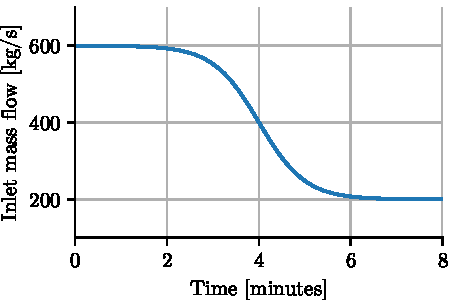
\includegraphics{figures/inlet_mass_flow.pdf}%
    \caption{%
        Plot of the inlet mass flow boundary condition, which simulates a transient occuring in a time span of approx 4~minutes.
        \label{fig:massFlowBoundaryCondition}%
    }%
\end{figure}%

% \begin{figure}[!ht]%
% \centering%
% \begin{minipage}{9.6cm}%
%     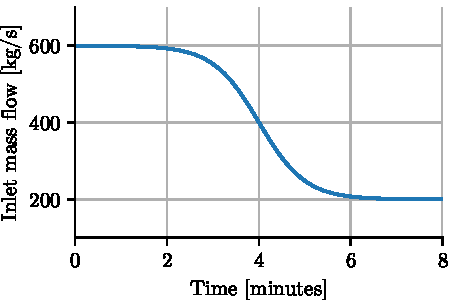
\includegraphics{figures/inlet_mass_flow.pdf}%
%     \caption{%
%         Plot of the inlet mass flow boundary condition, which simulates a transient occuring in a time span of approx 4~minutes.%
%         \label{fig:massFlowBoundaryCondition}%
%     }%
% \end{minipage}%
% \hspace{0.099cm}%
% \begin{minipage}{6.3cm}%
%     \caption{%
%         The gas.  composition used for the simulations.%
%         \label{tab:composition}%
%     }%
%     % \begin{tabular}{lc}
%     % \centering
%     % \begin{tabular}{lS}
%     \begin{tabular}{cl}%
%         \toprule
%         Component & {Mole fraction} \\ % use braces to protect from siunitx "S" alignment
%         \midrule
%         CH$_4$ & 0.8916 \\
%         C$_2$H$_6$ & 0.073513 \\
%         C$_3$H$_8$ & 0.005104 \\
%         iC$_4$H$_{10}$ & 0.000251 \\
%         nC$_4$H$_{10}$ & 0.000311 \\
%         iC$_5$H$_{12}$ & 0.000009 \\
%         nC$_5$H$_{12}$ & 0.000024 \\
%         N$_2$ & 0.006980 \\
%         CO$_2$ & 0.022208 \\
%         \bottomrule%
%     \end{tabular}
% \end{minipage}%
% \end{figure}%


The gas composition was kept fixed at the values shown in \cref{tab:composition}.
\begin{table}[!hb]
    \caption{
        The gas.  composition used for the simulations.
        \label{tab:composition}
    }
    % \begin{tabular}{lc}
    \centering
    % \begin{tabular}{lS}
    \begin{tabular}{cl}
        \toprule
        Component & {Mole fraction} \\ % use braces to protect from siunitx "S" alignment
        \midrule
        CH$_4$ & 0.8916 \\
        C$_2$H$_6$ & 0.073513 \\
        C$_3$H$_8$ & 0.005104 \\
        iC$_4$H$_{10}$ & 0.000251 \\
        nC$_4$H$_{10}$ & 0.000311 \\
        iC$_5$H$_{12}$ & 0.000009 \\
        nC$_5$H$_{12}$ & 0.000024 \\
        N$_2$ & 0.006980 \\
        CO$_2$ & 0.022208 \\
        \bottomrule
    \end{tabular}
\end{table}
%
% \begin{table}
%     \caption{
%         \redtext{Caption}
%         % \label{tab:composition}
%     }
%     \centering
%     \begin{tabular}{llllllllll}
%         \toprule
%         Component & CH$_4$ & C$_2$H$_6$ & C$_3$H$_8$ & iC$_4$H$_{10}$ &nC$_4$H$_{10}$ & iC$_5$H$_{12}$ & nC$_5$H$_{12}$ & N$_2$ & CO$_2$ \\
%         Mole fraction & 89.16 & 7.35 & 0.510 & 0.0251 & 0.0311 & 0.0009 & 0.0024 & 0.698 & 2.221 \\
%         \bottomrule
%     \end{tabular}
% \end{table}

\subsection{Sensitivity study}
Which parameters to include in the sensitivity study were determined by looking at which variables appear in the governing equations (\cref{eq:continuityEquation,eq:momentumEquation,eq:energyEquation}), in addition to other correlations that are used in the simulations. The focus was on simplifications and empirical correlations in the models, not on physical parameters like pipe diameter, ambient temperature, etc. %
The following nine parameters are included in the study:
\begin{itemize}
    \item the Colebrook-White correlation for the friction factor $f$, \cref{eq:colebrookWhite}
    
    \item the compressibility factor $Z$ and three derivatives: $\eval{\pd{Z}{T}}_p$, $\eval{\pd{Z}{p}}_T$ and $\eval{\pd{Z}{T}}_\rho$, which are all calculated from the equation of state
    
    \item Nusselt number relations (the Dittus-Boelter equation and \cref{eq:outerFilm}) for inner and outer film heat transfer coefficients ($h_\text{inner}$ and $h_\text{outer}$), which go into the calculation of the heat transfer between the gas and the surroundings $\Omega$
    
    \item the correlation for heat capacity of the gas at constant volume %
    %(derived from the equation of state) 
    $c_v$
    
    \item the Lee-Gonzales-Eakin correlation for the viscosity of the gas $\mu$, \cref{eq:LGE}, which mainly enters the simulations via the Reynolds number, $\Reyn = \frac{\rho u D}{\mu}$
 \end{itemize}

% To decide which parameters and relations to include in the sensitivity study we first looked to the governing equations \cref{eq:continuityEquation,eq:momentumEquation,eq:energyEquation}. Obvious choices are the compressibility factor $Z$ and derivatives, the friction factor $f$, the gas heat capacity $c_v$, and the heat transfer $\Omega$, which all appear directly in the partial differential equations. We find that the inner and outer heat transfer coefficients ($h_\text{inner}$ and $h_\text{outer}$) are the most relevant parameters to use to investigate the sensitivtity to changes in the heat transfer. We also include the correlation for viscosity (\redtext{LGE}).

% To investigate the sensitivity of the model a \emph{base case} was first established using standard model parameters. The simulation was then repeated with one parameter multiplied by a factor of 1.2, and the corresponding changes in the modelled flow, pressure, and temperature were recorded. To quantify the sensitivity for changes in the different parameters, both the maximum differences and the average differences from the base case was calculated. This was calculated both for the whole simulation period of 4 days, and for selected points of interest along the pipeline.

To investigate the sensitivity of the model a \emph{base case} was first established using standard model parameters and the boundary conditions described in \cref{subsec:pipeline}. The inlet flow rate transient was initiated at around 2 hours, and the pipeline was simulated for 104 hours after the transient.
%
The simulation was then repeated several times, with a different parameter modified by a constant factor of 1.2 each time. The corresponding response in the modelled flow, pressure, and temperature were recorded for each case. 

% To quantify the sensitivity for changes in the different parameters, both the maximum differences and the average differences from the base case was calculated, for the whole simulation period. 

% \section{Results and discussion}
\section{RESULTS AND DISCUSSION}
\label{results}
% The boundary conditions for the off-shore pipeline were inlet mass flow, outlet pressure, inlet temperature and inlet \co-concentration, see \cref{fig:offshorePipelineBC} for a plot of these. 
% The pipeline was simulated for a 14 day winter period and a 18 day summer period. 
% For the heat transfer model, sea bottom temperature and air temperature profiles along the pipeline that were sampled once per day were used as boundary conditions. The ambient sea bottom temperatures are from oceanographic models, and the air temperatures are expected temperatures based on historical measurements. \todo{Plot amb temp? 1 line per day, doable in 1 fig}


In \cref{fig:baseCaseWithZ} is a plot of the boundary conditions for the base case, and the results for a simulation where the compressibility factor $Z$ has been increased by \SI{20}{\percent}. 

% The biggest impact is on the inlet pressure, which is increased by up to \SI{7}{\percent}.

%In a simulation of a real pipeline, where measurements of the pressure etc. at the inlet and outlet are available, the pipeline roughness $\epsilon$ would typically have been tuned to match the measured pressure drop \todo{using data from a period of stable operation}. Here we have not tuned the roughness to match the base case pressure drop
% \begin{figure}[ht]%
%     \centering%
%     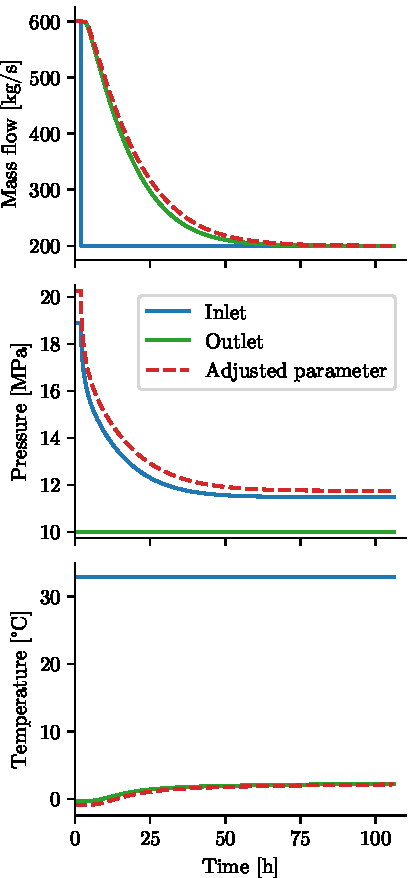
\includegraphics{figures/base_case_with_adjusted_Z.pdf}%
%     \caption{%
%         \redtext{Caption.} Inlet flow ramp down at 2 hours. Differences vary with time.
%         \label{fig:baseCaseWithZ}%
%     }%
% \end{figure}%
\begin{figure}[!ht]%
    \centering%
    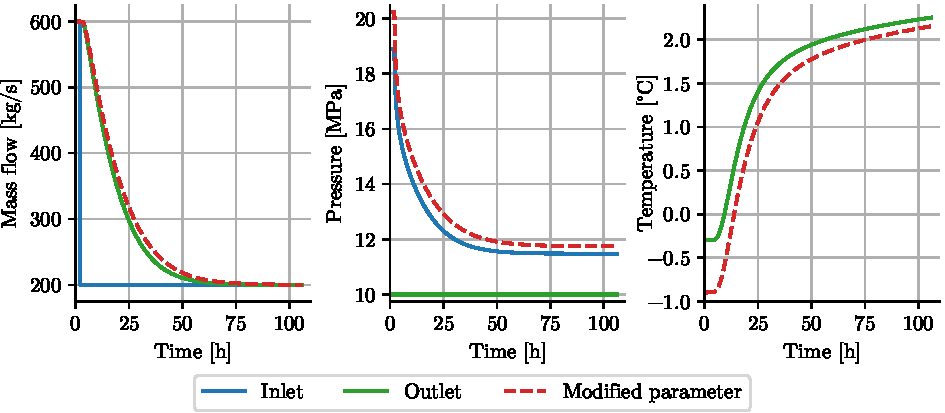
\includegraphics{figures/base_case_with_adjusted_Z_horiz.pdf}%
    \caption{%
        A plot of the results from the base case, and from a simulation with a modified parameter (the compressibility factor $Z$). The inlet flow rate transient occurs at 2~hours, and the boundary conditions are then kept constant for 104~hours. The constant inlet temperature of \SI{33}{\celsius} is not shown.
        \label{fig:baseCaseWithZ}%
    }%
\end{figure}%
From \cref{fig:baseCaseWithZ} it is clear that the differences vary with time during the transient%
, so to more easily analyze the results, both the time average relative difference
\begin{align}
    \overbar{\Delta y_\mathrm{rel}}
    = \frac{1}{n} \sum_{i=1}^n \Delta y_\mathrm{rel}
    = \frac{1}{n} \sum_{i=1}^n \frac{y_i - y_i^0}{y_i^0}
\end{align}
and the maximum relative difference
\begin{align}
    \max\del{\Delta y_\mathrm{rel}} = \max\del{\frac{y_i - y_i^0}{y_i^0}}
\end{align}
between the base case ($y^0$) and the simulations with modified parameters ($y$) was calculated, for mass flow, pressure and temperature. %
This was calculated for each parameter in the sensitivity study, at every grid point of the pipeline. Since a transient case is simulated, the relative differences are used, to normalize the differences. %
% For for mass flow and pressure the relative difference was used
% \begin{align}
%     \eval{\Delta y}_\textrm{relative} = \frac{y - y^0}{y^0}
% ,
% \end{align}
% while the absolute difference was used for temperature
% \begin{align}
%     \eval{\Delta y}_\textrm{absolute} = \abs{y - y^0}
% .
% \end{align}
%
% A plot of the maximum and average differences for the compressibility factor $Z$ can be seen in \cref{fig:maxAndAverageDiffForZ}, where the maximum and average mass flow, pressure, and temperature difference is shown for the whole pipeline. 
%
A plot of the maximum and average differences as function of position, for all parameters in the study, are shown in \cref{fig:maxAndAverageForAll}, and a list of the average impact on the whole pipeline is given in \cref{tab:averageImpact}. %

From \cref{fig:maxAndAverageForAll} a) and b) it can be seen that the parameters with the highest impact on both mass flow and pressure are the friction factor $f$ and the compressibility factor $Z$. For the mass flow the greatest impact is at the outlet, with a gradual decrease from the inlet to the outlet. For the pressure the greatest impact is at the inlet, with a gradual decrease from the inlet to the outlet. 
% All other parameters have %
% less than \SI{1.3}{\percent} maximum %
% %(\redtext{1.23 for dZdT|p}) %
% and less than \SI{0.3}{\percent} average %
% %(\redtext{0.278 for dZdp|T}) %
% impact on the mass flow, and %
% less than \SI{0.5}{\percent} maximum %
% % (\redtext{0.471 for viscosity}) %
% and \SI{0.4}{\percent} average %
% % (\redtext{0.337 for viscosity}) %
% impact on the pressure. %

% A list of the average impact of all parameters is listed in \cref{tab:averageImpact}. %
%
The average impact on mass flow is found to be \SI{1.43}{\percent} for the friction factor and \SI{0.90}{\percent} for the compressibility factor, % 6.5703443811 4.133998237
which is respectively 6.6 and 4.1 times higher than the third most important factor, $\eval{\partial Z/\partial p}_T$, which has an average impact of \SI{0.22}{\percent}. %
%
The average impact on pressure is \SI{3.09}{\percent} for the friction factor and \SI{2.07}{\percent} for the compressibility factor, % 14.3347939844 9.6177252345
which is respectively 14.3 and 9.6 times higher than the next most important factor, $\mu$, which has an average impact of \SI{0.20}{\percent}. %
%
% Further, peaks in several of the mass flow and temperature responses are seen between where the pipeline enters the ocean at \SI{25}{\kilo\meter} and \SI{50}{\kilo\meter}.

\begin{figure}[!p]%
    \centering%
    % 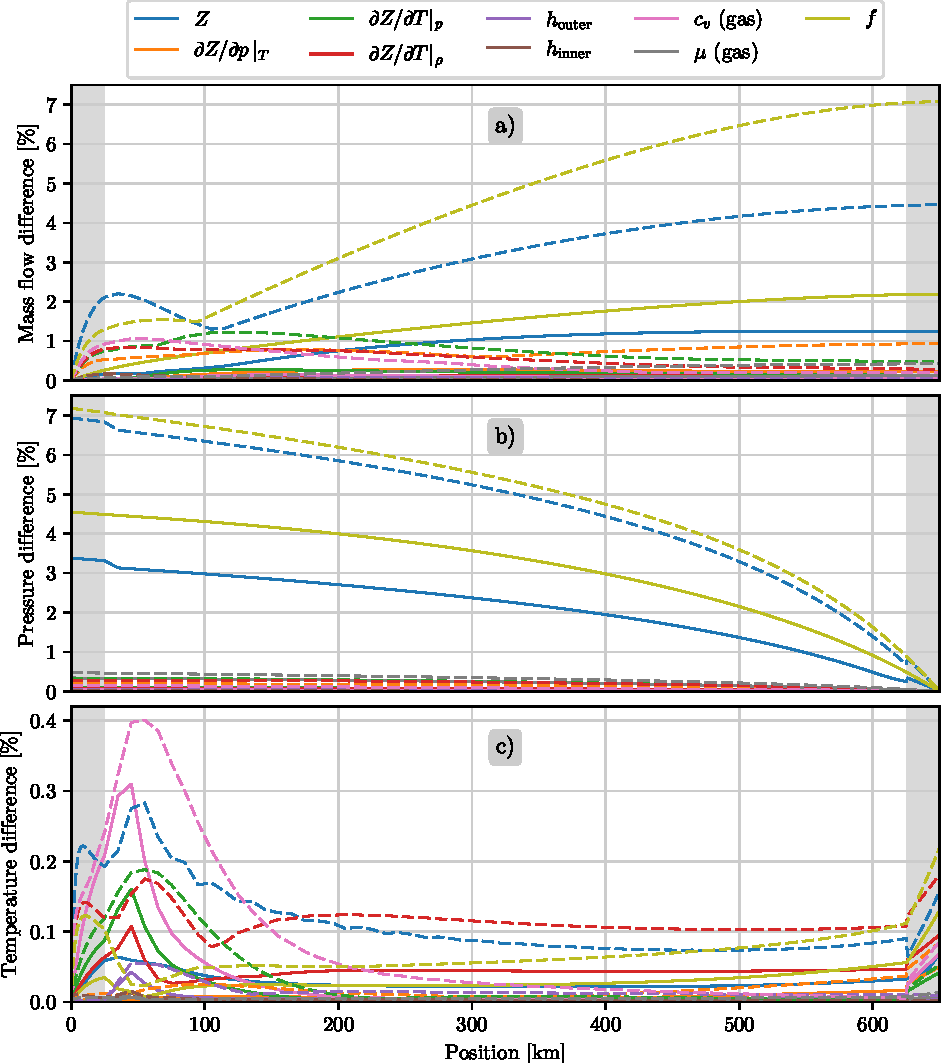
\includegraphics{figures/difference_along_pipeline_shaded_abc.pdf}%
    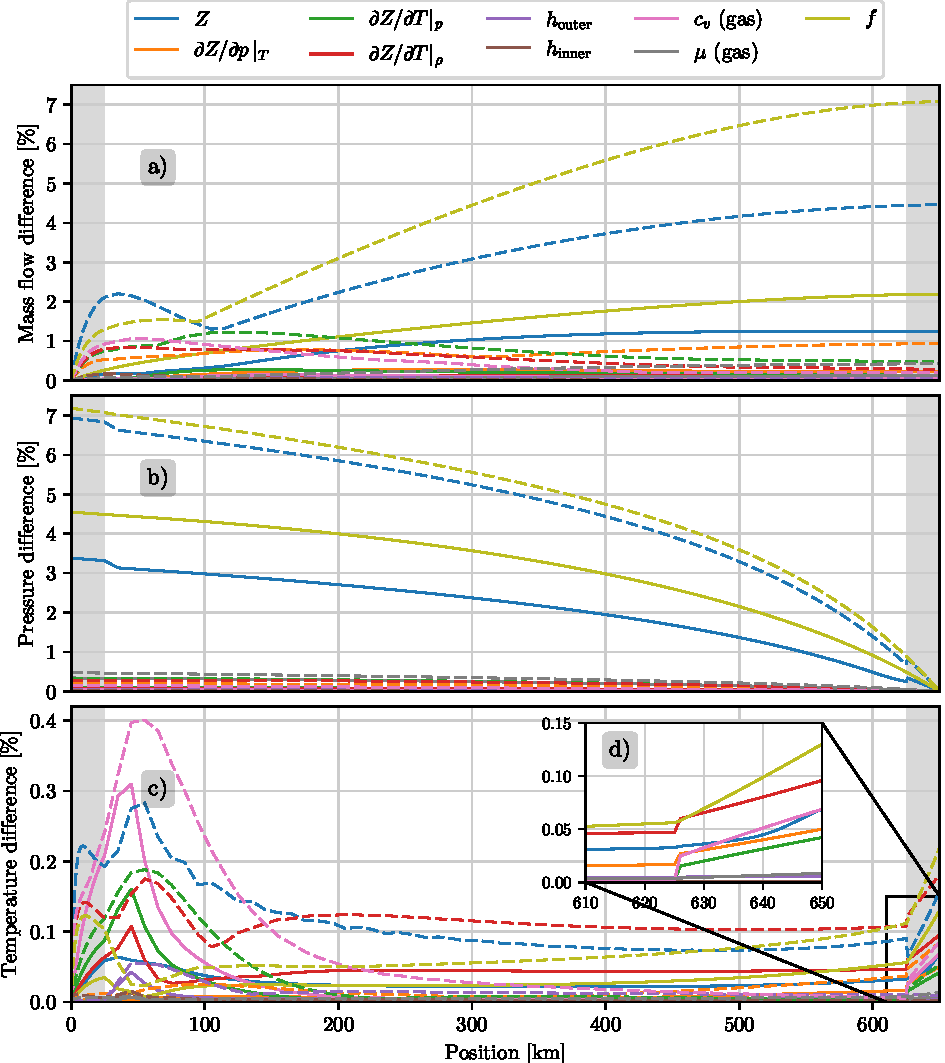
\includegraphics{figures/difference_along_pipeline_shaded_abc_inset.pdf}%
    \caption{%
        Plots of the maximum (dashed lines) and time average (solid lines) difference between the base case and the cases with a parameter increased by \SI{20}{\percent}, for each grid point used in the simulations. The gray shaded areas on the left and right side illustrate the on-shore parts of the pipeline.
        \label{fig:maxAndAverageForAll}%
    }%
\end{figure}%

\begin{table}[!hb]
    \caption{
        Table of the average relative difference in mass flow, pressure and temperature, for all parameters in the sensitivity study. \redtext{weighted average using non-uniform grid spacing} %
        % For mass flow and pressure the two highest numbers are highlighted in green, and the third-highest in yellow.
        \label{tab:averageImpact} %
    } %
    % \begin{tabular}{lc}
    \centering %
    % \begin{tabular}{lS}
    \begin{tabular}{cccc} %
        \toprule
        % Parameter & \parbox{3.3cm}{\centering Average \\ difference in \\ mass flow [\si{\percent}]} & \parbox{3.3cm}{\centering Average \\ difference in \\ pressure [\si{\percent}]} & \parbox{3.3cm}{\centering Average \\ difference in temperature [\si{\percent}]} \\
        & \multicolumn{3}{c}{Average relative difference} \\ \cmidrule(r){2-4}
        \parbox{2.5cm}{\centering Parameter} & Mass flow [\si{\percent}] & Pressure [\si{\percent}] & Temperature [\si{\percent}] \\
        \midrule
        % output from Python script goes here
        % relative temperature
        $Z$ & 0.9007 & 2.0722 & 0.0289 \\
        $\eval{\partial Z/\partial p}_T$ & 0.2179 & 0.0527 & 0.0084 \\
        $\eval{\partial Z/\partial T}_p$ & 0.1859 & 0.0614 & 0.0157 \\
        $\eval{\partial Z/\partial T}_\rho$ & 0.1021 & 0.0567 & 0.0454 \\
        $h_\mathrm{outer}$ & 0.0171 & 0.0073 & 0.0061 \\
        $h_\mathrm{inner}$ & 0.0033 & 0.0015 & 0.0015 \\
        $c_v$ (gas) & 0.0881 & 0.0225 & 0.0321 \\
        $\mu$ (gas) & 0.0782 & 0.2155 & 0.0027 \\
        $f$ & 1.4316 & 3.0885 & 0.0306 \\
        \bottomrule
    \end{tabular}
\end{table}

% % \begin{table}[ht]
%     \begin{center}
%         \begin{tabular}{RRRRRRRRRR}
%           1.00 & 1.00 & 1.00 & 1.00 & 0.99 & 0.98 & 0.96 & 0.90 & 0.82 & 0.37 \\
%           1.00 & 1.00 & 0.99 & 0.98 & 0.95 & 0.90 & 0.82 & 0.61 & 0.37 & 0.01 \\
%           1.00 & 0.99 & 0.98 & 0.96 & 0.90 & 0.82 & 0.67 & 0.37 & 0.14 & 0.00 \\
%           1.00 & 0.98 & 0.95 & 0.90 & 0.78 & 0.61 & 0.37 & 0.08 & 0.01 & 0.00 \\
%           0.99 & 0.95 & 0.90 & 0.82 & 0.61 & 0.37 & 0.14 & 0.01 & 0.00 & 0.00 \\
%           0.98 & 0.90 & 0.82 & 0.67 & 0.37 & 0.14 & 0.02 & 0.00 & 0.00 & 0.00 \\
%           0.95 & 0.78 & 0.61 & 0.37 & 0.08 & 0.01 & 0.00 & 0.00 & 0.00 & 0.00 \\
%           0.90 & 0.61 & 0.37 & 0.14 & 0.01 & 0.00 & 0.00 & 0.00 & 0.00 & 0.00 \\
%           0.82 & 0.37 & 0.14 & 0.02 & 0.00 & 0.00 & 0.00 & 0.00 & 0.00 & 0.00 \\
%           0.37 & 0.01 & 0.00 & 0.00 & 0.00 & 0.00 & 0.00 & 0.00 & 0.00 & 0.00 \\
%         \end{tabular}
%     \end{center}
% \end{table}

\begin{table}[!hb]
    \caption{
        \redtext{caption}
        \label{tab:}
    }
    \centering
    \begin{tabular}{lRRT}
        \toprule
         % & \multicolumn{3}{c}{Item} \\
        & \multicolumn{1}{c}{Chemical Component} \\% & \parbox{4cm}{\centering Average relative impact on pressure} & \parbox{4cm}{\centering Average impact on temperature} \\
        % Parameter & [\si{\percent}] & [\si{\percent}] & [\si{\celsius}] \\
        \midrule
        % output from Python script goes here
        $Z$ & 0.8058 & 1.9431 & 0.0925 \\
        $\eval{\partial Z/\partial p}_T$ & 0.1769 & 0.0483 & 0.0371 \\
        $\eval{\partial Z/\partial T}_p$ & 0.1414 & 0.0562 & 0.0749 \\
        $\eval{\partial Z/\partial T}_\rho$ & 0.0852 & 0.0503 & 0.1400 \\
        $h_\mathrm{seawater}$ & 0.0134 & 0.0064 & 0.0132 \\
        $h_\mathrm{inner}$ & 0.0030 & 0.0013 & 0.0035 \\
        $c_v$ (gas) & 0.0676 & 0.0214 & 0.1579 \\
        Viscosity & 0.0724 & 0.1985 & 0.0087 \\
        Friction & 1.3207 & 2.7952 & 0.1160 \\
        \bottomrule
    \end{tabular}
\end{table}

For the temperature the situation is less clear-cut. From \cref{tab:averageImpact} it is seen that the parameter which gives the highest average difference along the whole pipeline is the derivative of the compressibility factor $\eval{\partial Z/\partial T}_\rho$, with an average difference of \SI{0.045}{\percent}, 1.41~times the impact of the next parameter ($c_v$) and 1.48~times the impact of the third parameter ($f$). Compared to mass flow and pressure, where the two parameters with the highest impact give a difference of between 4 and 14 times the parameter with the third highest impact, the numbers for the temperature seem to \redtext{vary less}.

Further, in \cref{fig:maxAndAverageForAll} c) peaks in the temperature responses of up to \SI{0.31}{\percent} are observed around \SI{20}{\kilo\meter} off-shore, before the impact of all parameters steadily decrease until they stabilize around \SIrange{100}{200}{\kilo\meter} off-shore. It can also be seen that between \SI{125}{\kilo\meter} (\SI{100}{\kilo\meter} off-shore) and landfall at \SI{625}{\kilo\meter}, all parameters have much lower impact than closer to the start of the pipeline; no parameter have a higher maximum impact than \SI{0.15}{\percent} or an average impact of more than \SI{0.06}{\percent}. %
The stable behaviour in this area is caused by the fixed sea temperature, which acts as a thermal reservoir, so after a long off-shore section the gas comes to a thermal equilibrium with the sea water, and the gas temperature is governed by the ambient temperature.
% This is because, after being transported offshore for some time, the gas comes to a thermal equilibrium with the ambient sea water. The sea has fixed temperature, and acts as a thermal reservoir, so after a long off-shore section the gas temperature will be governed by the ambient temperature, 
% and will be independent of any parameters that affect the heat exchange rate between the gas and the ambient (\redtext{as long as the heat exchange rate is different from zero})\todo{what about things like Joule Thompson?, are there other effects??}.

Finally, there is a steady increase in the impact on temperature between landfall and the outlet for most parameters. This is because at landfall the boundary conditions for the thermal exchange between the gas and the ambient changes (the pipeline goes from being exposed to sea water to buried under ground), and the thermal equilibrium between the gas and the ambient is disturbed. %Here the parameters that affect the heat exchange, like the inner and outer heat transfer coefficients, will again come into play
%
Some details on the temperature response near the outlet can be seen in the inset in \cref{fig:maxAndAverageForAll} d). It is clear that some of the parameters that have very little effect on the temperature while off-shore, like the heat capacity $c_v$ and the derivative of the compressibility factor $\eval{\partial Z/\partial T}_p$, have a much higher effect after going on-shore, and on the final outlet temperature. The impact of the derivative of the compressibility increases from \SI{0.0012}{\percent} at \SI{625}{\kilo\meter} to \SI{0.042}{\percent} at the outlet, a factor of 12.9, and the heat capacity $c_v$ increases from \SI{0.0018}{\percent} at \SI{625}{\kilo\meter} to \SI{0.069}{\percent} at the outlet, a factor of 13.8. The trend in the plot indicates that the impact would be even bigger with a longer on-shore section.

% \begin{figure}[!ht]%
%     \centering%
%     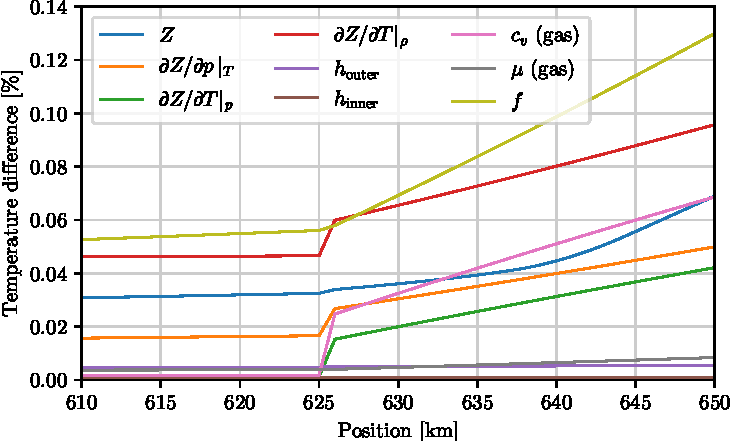
\includegraphics{figures/outlet_temperature_detail.pdf}%
%     \caption{%
%         Details of the response in temperature to changes in the different parameters, close to the outlet. Plot of the average temperature difference at each grid point.
%         % Plots of the maximum (dashed lines) and time average (solid lines) difference between the base case and the cases with a parameter increased by \SI{20}{\percent}. The gray shaded areas illustrate the on-shore parts of the pipeline.
%         \label{fig:outletTemperatureDetail}%
%     }%
% \end{figure}%

% \begin{figure}[!hb]%
%     \centering%
%     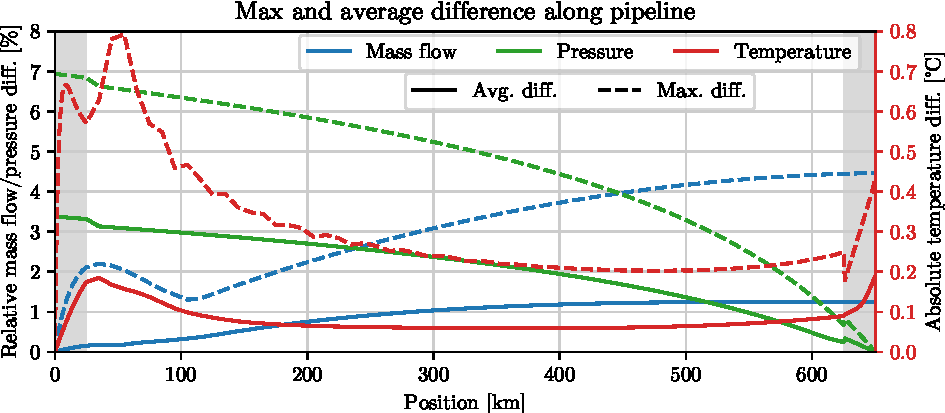
\includegraphics{figures/all_differences_position.pdf}%
%     \caption{%
%         The maximum (dashed lines) and time average (solid lines) difference between the base case and the results from the case with the compressibility factor $Z$ increased by \SI{20}{\percent}. Relative difference is used for mass flow and pressure (the left axis), and absolute difference for temperature (the right axis). The gray shaded areas illustrate the on-shore parts of the pipeline. \redtext{Not sure if this figure is necessary}
%         \label{fig:maxAndAverageDiffForZ}%
%     }%
% \end{figure}%

% In \cref{fig:massFlowBarChart,fig:pressureBarChart,fig:temperatureBarChart} the maximum and average differences between the base case and each case with modified parameters, at certain points of interest along the pipeline, are shown in bar charts. For the mass flow and pressure the observations from before are confirmed: the most important parameters are the friction factor $f$ and the compressibility factor $Z$, at the start of the pipeline for the pressure, and at the end of the pipeline for the mass flow.
%, like the inlet, the end of the on-shore section etc

To further analyze the temperature responses, the maximum and average temperature differences at certain points of interest along the pipeline are shown in a bar chart in \cref{fig:temperatureBarChart}. %
It is seen that the heat capacity $c_v$ is the parameter with the highest impact between all the selected points on the pipeline, with the two highest average temperature differences (respectively at \SI{20}{\kilo\meter} off-shore, and at the end of the on-shore section), and the highest and third highest maximum differences (respectively at \SI{20}{\kilo\meter} off-shore and at the end of the on-shore section). The parameter with the highest \st{average and maximum} impact at \SI{300}{\kilo\meter} offshore is the derivative of the compressibility factor $\partial Z/\partial T\/|_\rho$, while at the end of the off-shore section and at the outlet it is the friction factor $f$.

% It can be seen that for the first 45 kilometers of the pipeline, the most important
% parameter is the heat capacity $c_v$, giving an average temperature difference of up to \SI{0.87}{\celsius} (maximum difference of \SI{1.14}{\celsius}). Following this, in descending order of importance are the derivatives of the compressibility %
% $\eval{\partial Z/\partial T}_p$ %
% % $\eval{\pd{Z}{T}}_p$%
%  and %
% $\eval{\partial Z/\partial T}_\rho$%
% % $\eval{\pd{Z}{T}}_\rho$%
% ; and finally the compressibility itself, $Z$, with
% average temperature difference of up to \SI{0.45}{\celsius} (maximum difference of \SI{0.78}{\celsius}). %

% \begin{figure}[!p]%
%     \centering%
%     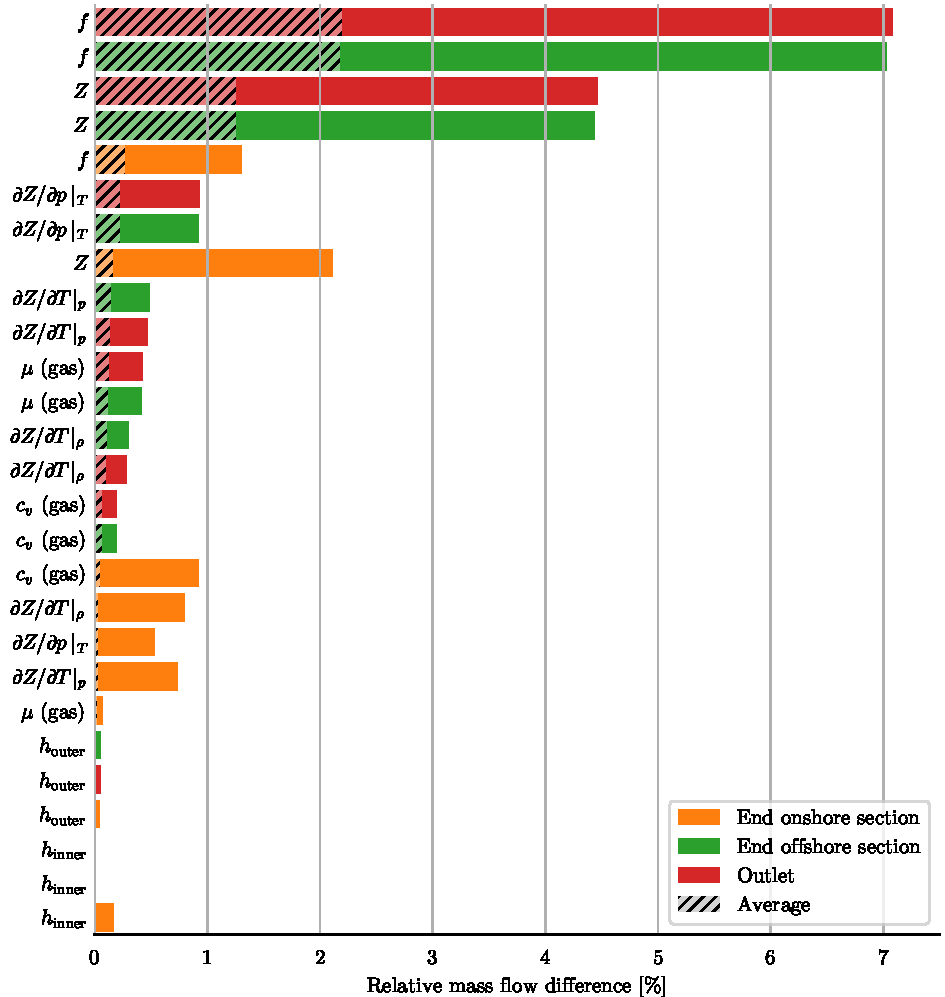
\includegraphics{figures/barchart_all_mass_flow_relative.pdf}%
%     \caption{%
%         Chart of the average and maximum relative difference in mass flow between the base case and the cases with modified parameters, for 3 different points on the pipeline (the end of the onshore section, the end of the offshore section, and the outlet). The bars are sorted by descending average error. 
%         %Only parameters/points with average relative difference above \SI{0.04}{\percent} are shown.%
%         \label{fig:massFlowBarChart}%
%     }%
% \end{figure}%

% \begin{figure}[!p]%
%     \centering%
%     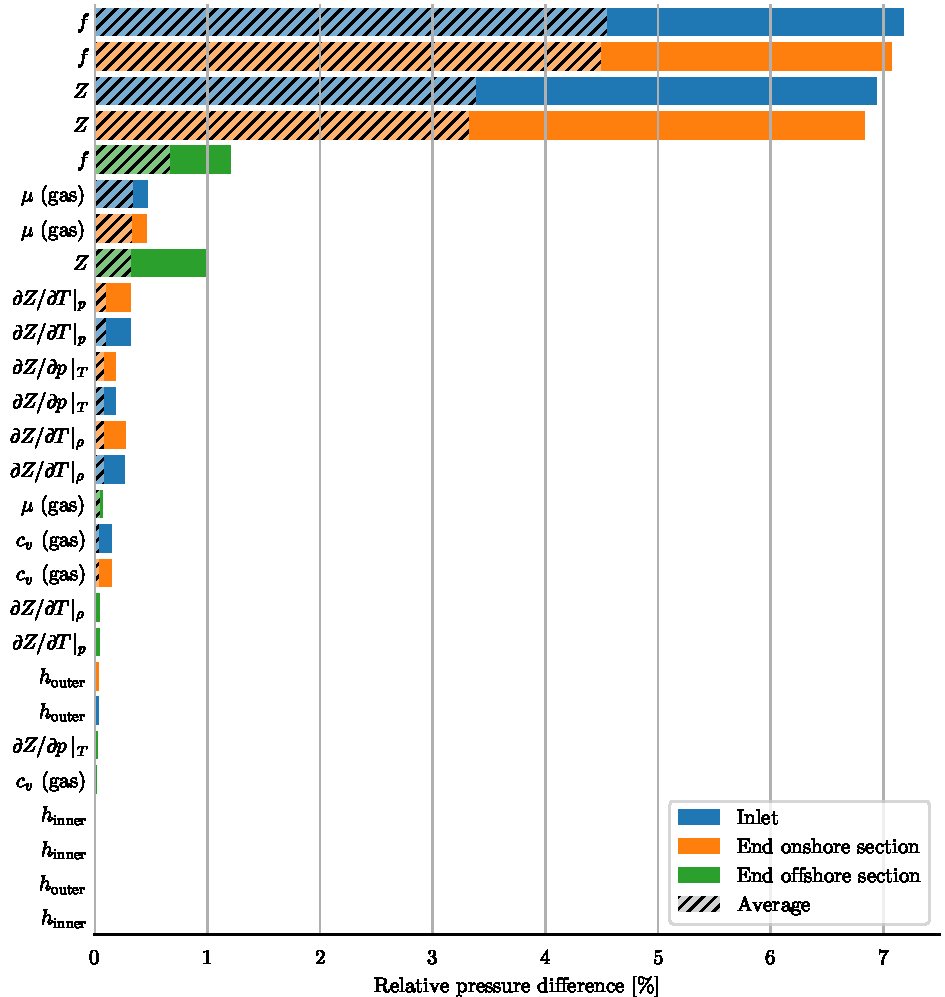
\includegraphics{figures/barchart_all_pressure_relative.pdf}%
%     \caption{%
%         Chart of the average and maximum relative difference in pressure between the base case and the cases with modified parameters, for 3 different points on the pipeline (the inlet, the end of the onshore section and the end of the offshore section). The bars are sorted by descending average error. 
%         %Only parameters/points with average relative difference above \SI{0.04}{\percent} are shown.%
%         \label{fig:pressureBarChart}%
%     }%
% \end{figure}%

\begin{figure}[!p]%
    \centering%
    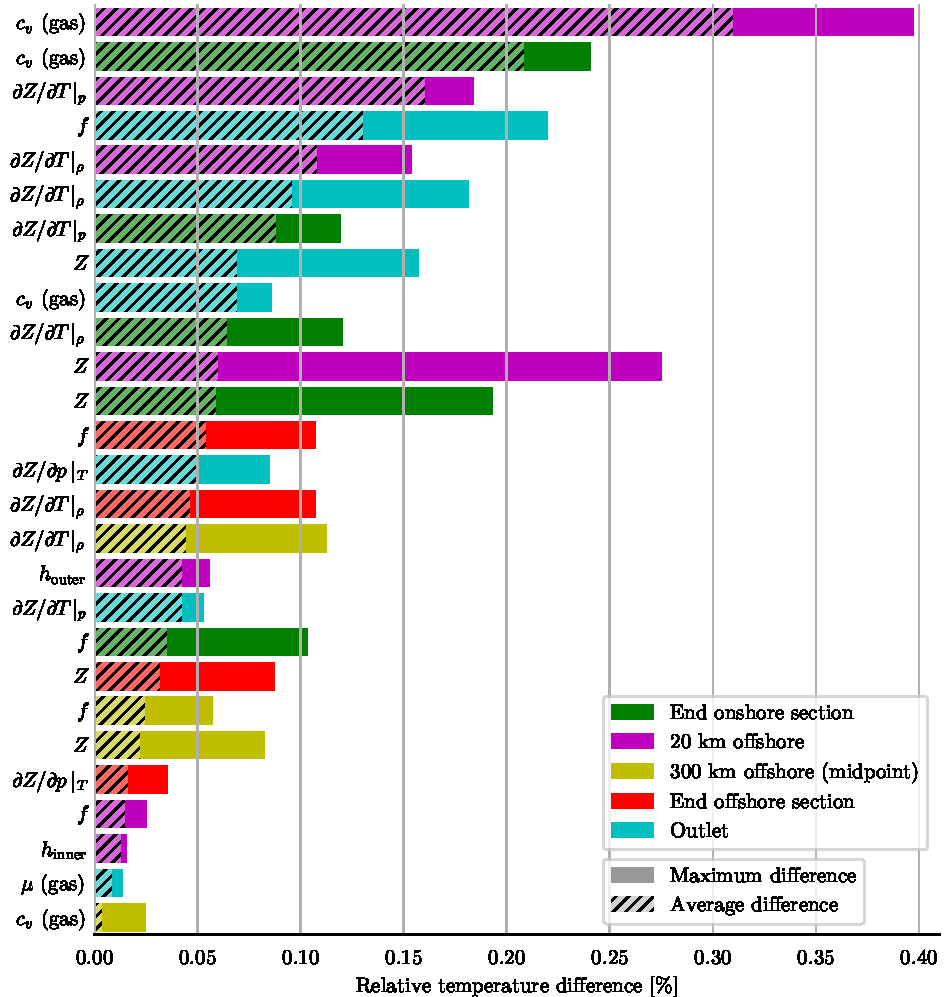
\includegraphics{figures/barchart_all_temperature_absolute.pdf}%
    \caption{%
        Chart of the average and maximum relative difference in temperature between the base case and the cases with modified parameters, for 5 different points on the pipeline (the end of the onshore section, \SI{20}{\kilo\meter} off shore, \SI{300}{\kilo\meter} off shore, and the end of the offshore section). The bars are sorted by descending average error. 
        Only parameters/points with average relative difference above \SI{0.0036}{\percent} are shown.%
        % cut-off at average absolute difference $>0.0371$ C.
        \label{fig:temperatureBarChart}%
    }%
\end{figure}%

% \begin{figure}[ht]%
%     \centering%
%     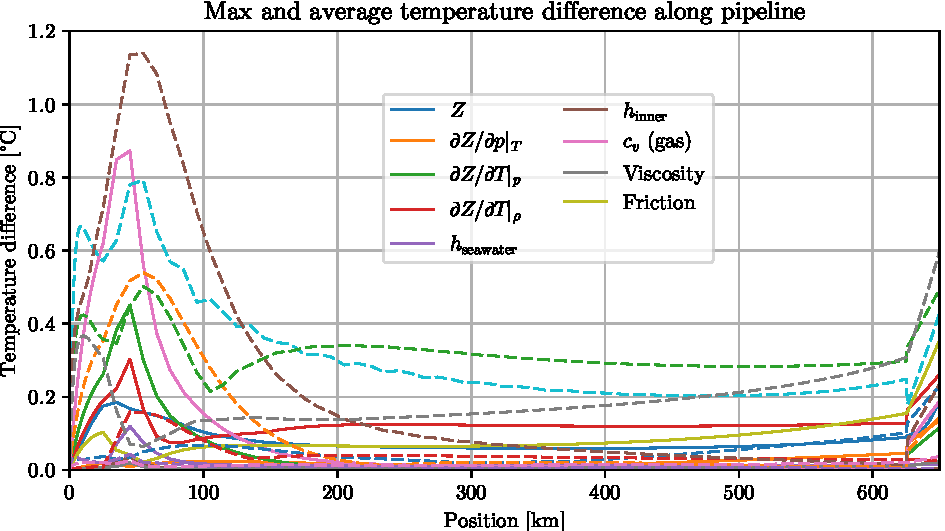
\includegraphics{figures/temperature_difference_along_pipeline.pdf}%
%     \caption{%
%         \redtext{Consider making a graph like this for mass flow and pressure as well? Could possibly make a page heigh subfigure thing.}
%         \label{fig:}%
%     }%
% \end{figure}%

% \begin{figure}[h]%
%     \centering%
%     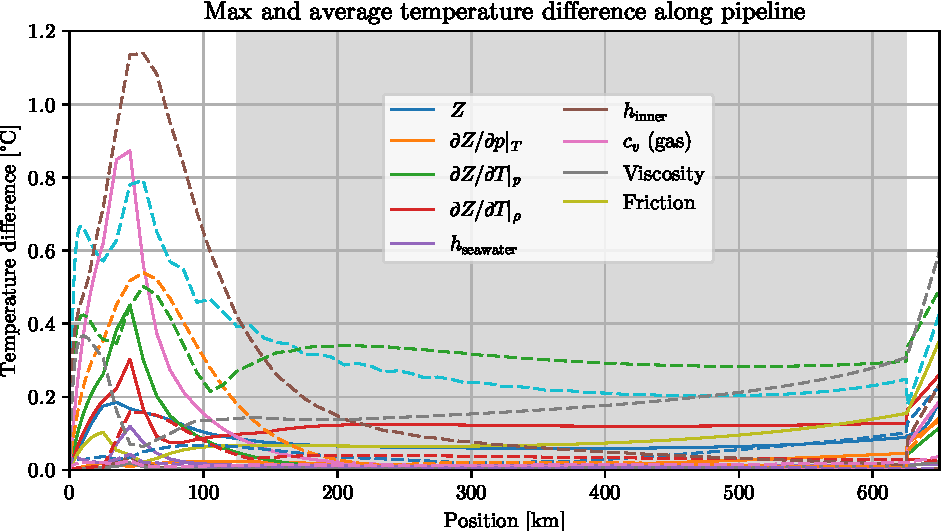
\includegraphics{figures/temperature_difference_along_pipeline_shaded.pdf}%
%     \caption{%
%         \redtext{Caption.}
%         \label{fig:}%
%     }%
% \end{figure}%

% \section{Conclusions}
\section{CONCLUSIONS}
\label{conclusion}
\begin{table}[!hb]
    \caption{
        \redtext{caption}
        % For mass flow and pressure the two highest numbers are highlighted in green, and the third-highest in yellow.
        % \label{tab:averageImpact}
    }
    % \begin{tabular}{lc}
    \centering
    % \begin{tabular}{lS}
    \begin{tabular}{lclcc}
        \toprule
        % Parameter & \parbox{4cm}{\centering Average relative impact on mass flow [\si{\percent}]} & \parbox{4cm}{\centering Average relative impact on pressure [\si{\percent}]} & \parbox{4cm}{\centering Average impact on temperature [\si{\celsius}]} \\
        Parameter & \multicolumn{2}{c}{\parbox{4cm}{\centering Average relative impact on mass flow [\si{\percent}]}} & \parbox{4cm}{\centering Average relative impact on pressure [\si{\percent}]} & \parbox{4cm}{\centering Average impact on temperature [\si{\percent}]} \\
        \midrule
        $Z$ & 0.8058 & \colorbox{green}{\hspace{0.8058cm}} & 1.9431 & 0.0329 \\
        $\eval{\partial Z/\partial p}_T$ & 0.1769 & \colorbox{green}{\hspace{0.1769cm}} & 0.0483 & 0.0134 \\
        \bottomrule
    \end{tabular}
\end{table}

\section*{Acknowledgements}
This work has been funded by the Norwegian gas operating company Gassco as part of a project to improve flow modeling in offshore natural gas transmission pipelines. 

\printbibliography
\end{document}